\documentclass[conference]{IEEEtran}
%\documentclass[journal]{IEEEtran}
%\usepackage{algorithmic}
%\usepackage{graphicx}
\usepackage{epsfig}
\usepackage{color}
\usepackage{array}
\usepackage{amsmath}
\usepackage{fontenc}
\usepackage{textcomp}
\usepackage{amsthm}
%\usepackage{url}
\usepackage{balance}
\usepackage{algorithm}
\usepackage{algpseudocode}
\usepackage{pifont}
\usepackage{nth}
%\usepackage{mathtools}

\newtheorem{mydef}{Definition}
\newtheorem{myex}{Example}
%\usepackage[lined,  ruled, linesnumbered]{algorithm2e}

\makeatletter

%%%%%%%%%%%for copyright notice
\def\ps@IEEEtitlepagestyle{%
    \def\@oddfoot{\mycopyrightnotice}%
    \def\@evenfoot{}%
}
\def\mycopyrightnotice{%
    {\footnotesize  978-1-5386-0869-2/17/\$31.00 \textcopyright2017 IEEE\hfill}
    \gdef\mycopyrightnotice{}
}
%%%%%%%%%%%

\makeatletter
\newcommand{\algrule}[1][.1pt]{\par\vskip.5\baselineskip\hrule height #1\par\vskip.5\baselineskip}
\makeatother

\makeatletter
\newcommand*\titleheader[1]{\gdef\@titleheader{#1}}
\AtBeginDocument{%
  \let\st@red@title\@title%
  \def\@title{%
    \bgroup\normalfont\small\raggedright\@titleheader\par\egroup
    \vskip1.5em\st@red@title}
}
\makeatother


\ifCLASSINFOpdf
 
\else
  % or other class option (dvipsone, dvipdf, if not using dvips). graphicx
  % will default to the driver specified in the system graphics.cfg if no
 
  % \DeclareGraphicsExtensions{.eps}
\fi
% correct bad hyphenation here
\hyphenation{op-tical net-works semi-conduc-tor}

\title{Smart Disaster Notification System}
\titleheader{Proceedings of the 2017 4th International Conference on Advances in Electrical Engineering (ICAEE),\\ 28-30 September, Dhaka, Bangladesh}

\begin{document}
%
% paper title
% can use linebreaks \\ within to get better formatting as desired




\author{\IEEEauthorblockN{Md. Fahim Sikder$^{1,a}$, Sajal Halder$^{2,b}$, Tanvir Hasan$^{3,c}$, Md. Jamal Uddin$^{4,c}$ and Mrinal Kanti Baowaly$^{5,c}$}
\IEEEauthorblockA{Department of Computer Science and Engineering}
\IEEEauthorblockA{$^{a}$Jahangirnagar University, Bangladesh}
\IEEEauthorblockA{$^{b}$Jagannath University, Bangladesh}
\IEEEauthorblockA{$^{c}$Bangabandhu Sheikh Mujibur Rahman Science and Technology University, Bangladesh} 
\IEEEauthorblockA{E-mail: fahimsikder01@gmail.com$^{1}$, sajal@cse.jnu.ac.bd$^{2}$, tanvir.bsmrstu@gmail.com$^{3}$, jamal.bsmrstu@gmail.com$^{4}$,\\ baowaly@gmail.com$^{5}$}
}

% make the title area
\maketitle


\begin{abstract}
%\boldmath
The devastations of natural disasters are the lash of mother nature that every year hit us with a whip. They are inevitable. There are no alternative ways to prevent this incident, but we can take proper steps to reduce its damage. Now-a-days a great deal of attention is given to the potential of mobile communication technology. Short Message System (SMS) has a huge impact on the communication system. This paper proposes an android application which should alert people before a natural disaster such as cyclone and flood, and tell them the optimal route to the nearest shelter via SMS or voice call. In evacuation process, we use partition based shortest technique to find nearest shelter place. %It is very faster than state of the art methods. 

\end{abstract}

\begin{IEEEkeywords}
Natural Disaster, Notification System, Android, Location Based, Nearest Shelter
\end{IEEEkeywords}

\IEEEpeerreviewmaketitle
\section{Introduction}
\label{sec:Intro}

Natural disasters are the consequences of natural hazards. It does occur a serious breakdown in the sustainability of  human, animals and property. It also occurs economic losses and disruption of economic and social progress. The overwhelming number of dead or seriously injured and homeless people are affected by the occurrence of a natural disaster. The massive amount of money to be spent for reconstruction and rehabilitation equates to a natural disaster. They are nothing else but extreme environmental events that impact human activities. Hurricane, Earthquakes, Tsunamis and volcanic eruptions are the most frequent threats as well as flooding \cite{khalid2015flood}, tornadoes and droughts which are also prevalent.
    
According to the “Annual Disaster Statistical Review 2010” \cite {guha2011annual}, 330 natural disasters were registered worldwide in 2003. Within that, there has been a total of 21,610 people who have been killed where the number of people killed by floods was 9,819 and the number of these killed by storms were 8583. And the estimated damage was 118.6 billion dollar. The statistics only got worse. But the worst part really is that there is no way of preventing natural disaster. The only way we can survive these is preparing for what may come.
 
Researchers had tried to give early warning system to minimize the loss. They came up with some brilliant way to do it \cite{zimmers2015alert,fajardo2010implementation,lo2015developing}. In this modern time mobile have really changed the way of communications \cite{laird2007mobile,rahman2012location}. It is the most used communication tools. Some of them tried to use Short Message System (SMS)\cite{mahmud2012sms} as an alerting system for the disaster. SMS is used on modern handsets originated from radio telegraphy \cite{turner2013wireless} in radio memos pagers using standardized phone protocols. These are defined as the part of the Global System for Mobile Communications (GSM) series \cite{waidyanatha2007challenges} of standards as a means of sending messages up to 160 characters to and from GSM supported devices. But by this method there is no way of evaluating the level of the disaster because no databases are used. This method only sends messages to the subscribers. But subscriber could be blind, so this method would not be helpful for blind people. Again, researchers used android technology \cite{fajardo2010implementation} to easy the system. They used algorithm to calculate optimal routes to the shelter for evacuation at the time of disaster and showed the data into google map.

Our proposed technique is an android based application which takes weather updates from websites and calculates the disaster level. Subscriber’s data can be stored in this application’s database. It can calculate the optimal route to the shelter from the subscriber’s current position and send voice call/ SMS with warning and shelter location to them. It sends voice call or voice alarm so blind subscriber can also get the alert. This is GSM type alerting system so subscriber do not need to have an android device in order to receive the service. It also stores previous weather statistics data in the database. Using these data and real-time data, it can predict upcoming weather by using machine learning techniques. Here it uses Naïve Bayes algorithm \cite{wiki:naive} to predict weather by analyzing the previous and real-time data. 

The remaining sections of the paper are organized as follows. In section \ref{relatedworks} describes related work on disaster notification systems. Section \ref{sec:problem} introduces our proposed smart disaster notification model. Implementation of our proposed technique has been described in section \ref{implementation}. Result analysis has been shown in section \ref{result}. Application of the systems and discussion as well as the future researches are shown in section \ref{conclusion}.
  
\begin{figure*}[htp]
	\centering
		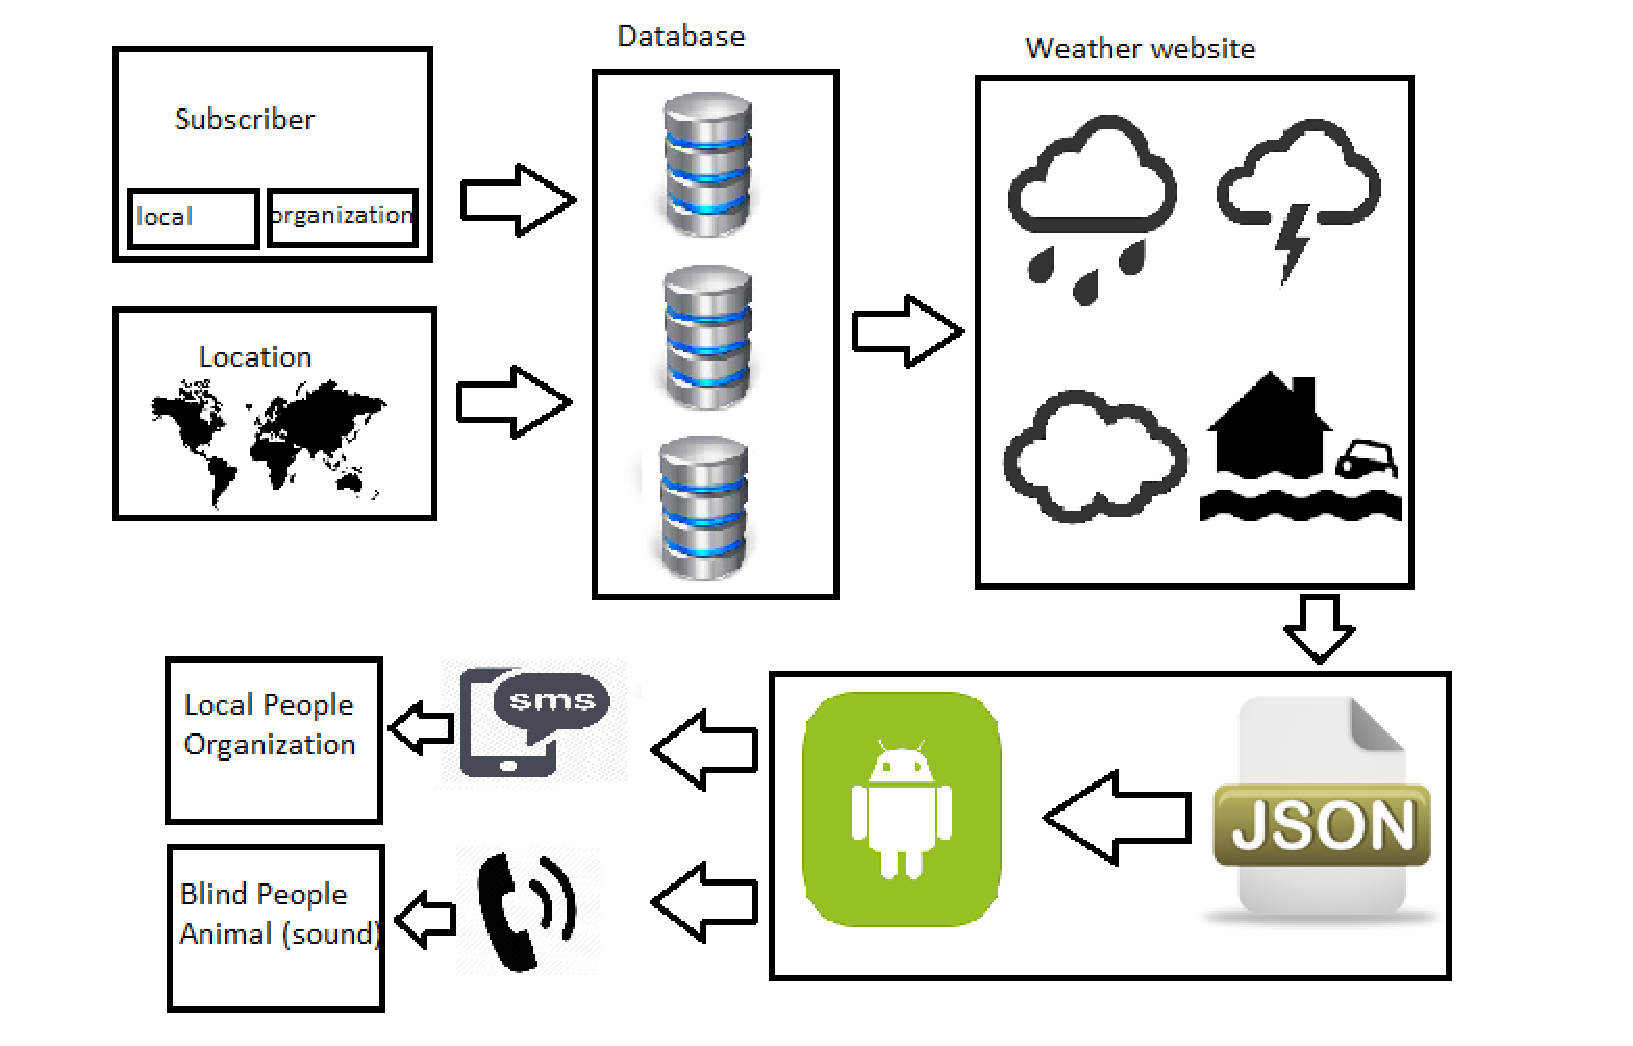
\includegraphics[width=.95\textwidth]{fig/architecture.eps}
	\caption{ System Overview }
	\label{Figure:overview}
\end{figure*}


\section {Related Work}
\label {relatedworks}

Early disaster warning and evacuation approach are very general disaster management system in disaster-prone areas. Nowadays mobile phones play an essential role in disaster management system in several ways: monitoring, communicate, warning dissemination, evacuation and rescue and relief aid. A number of notification system has been proposed in our real world. In research paper \cite{cioca2008sms, jeong2009national}, Short Message Service (SMS) is sent to all citizens from the server about the awareness of upcoming flood warning. A huge number of SMS transfer from the server cause network congestion and can break the voice communication system in the same network. To avoid this kind of congestion cell broadcasting service is used to directly send messages to the subscribers in a specific area \cite {scherner2005notifying}. But this process fails to help in evacuation process which provides information about the safe region. GSM alarm device is used for evacuation process in which three kinds of warning are sent to the police station or fire brigade station \cite{jayasinghe2006gsm}. Although it can avoid network congestion, the GSM alarm is not a faster way for evacuation process.  
 
Satellite communication systems will be very fast, reliable and robust. As a result, well-developed countries like Australia and South Korea are planning to use satellite communication for disaster management \cite{park2006one, aloudat2011toward,jeong2009national}. This satellite service maintenance is expensive and developing countries cannot afford this. Very few researchers propose location based services for disaster management on mobile phones. Previous works on location based services for disaster management did not distinguish normal people and blind people. Considering this, Amit Gosavi et. al. \cite{amit2014} presented a location based early warning and evacuation system by visual and audio warnings useful to both normal and blind people. 

Natural Disasters such as cyclone, storm, earthquake, Tsunami, and flood have shown the harmful, damaging mode of nature which has taken millions of lives including people and animals. Above all techniques are concern about people warning. Most of them did not discuss evacuation processes by which people get shelter place. Dijkstra's algorithm based shortest path calculation is used to find the nearest shelter place\cite{amit2014}. This process is time-consuming because it searches all paths from the source to destination. For this, we propose a location based smart disaster management system that can warn all subscribers (people, blind people). In the evacuation process, we used partition based trajectory to find nearest shelter place. It is very faster than the previously proposed methods.  

\section {Proposed Solution}
\label{sec:problem}

The main purpose of “Smart Disaster Notification System” is to alert people before the time of disaster and tell them the optimal route to the nearest shelter. In our system, we divide the whole application in some module. First one is database building that consists of subscriber information and locations whose probability of disaster is measured. The second one is based on locations in which our proposed methods take information from the weather website. After that these information will be converted to JSON (JavaScript Object Notation) \cite{bray2014javascript} format. Then,  according to JSON information, the system will be able to understand the probability of disaster and then the system will send nearest shelter information to the subscribers. The architecture of our proposed technique depicts in figure \ref{Figure:overview}. Each part of our system will be explained details in the next few sections. 

\subsection{Preliminaries}
\label{preliminaries}

The consequence of natural hazards is called the natural disaster. There are different kinds of natural disaster such as cyclone, storm, earthquake, Tsunami and flood etc. Different kinds of natural disaster occurs at the different time in different geographical area. Some recent examples of violent natural disasters are the 2011 Japan earthquake and Tsunami, the 2010 Haiti earthquake, the 2007 cyclone SIDR, the 2004 Indian Ocean Tsunami, the 1991 Bangladesh cyclone. Geographically few South Asian countries are situated in between the Himalayas and the ocean, on the delta of wide rivers, means that the countries are very exposed to flooding \cite{latif2011openstreetmap}.  The people live in coastal areas have to face several storms each year and cultivable lands disappear in the river due to river erosion. Such countries are mostly affected by the planet’s climate changes and number of cyclones. Hence, there is also the risk of Tsunami in these countries. Our disaster preparedness system protects the people from upcoming disaster. For this it uses SMS, voice call or voice alert. Our proposed work can be implemented on android mobile phones. Android \cite{developers2011android} is an operating system for mobile devices such as smart phones and tablet computers developed by Open Handset Alliance led by Google. As android is more open and comprehensive than other mobile operating system, this is the best selling product worldwide. It also allows building of new applications at lower cost. Consequently, this is more interactive for users. Hence, an android mobile platform has been used in our proposed disaster awareness system.


\subsection{Input into database}

We will keep the record of subscribers in the database. In there we will store the subscriber name, location and mobile number. Based on the subscriber locations we can give them the proper warning about the disaster. Smart disaster notification system will fetch the information from it and sends notification to the subscribers. Sending notification will depend on update from the websites.



\subsection{Update from website}
This application will take update from website and evaluate the level of disaster. Then it will convert the data into JSON format. The following figure \ref{Figure:update} shows the update process.

\begin{figure}[htp]
	\centering
		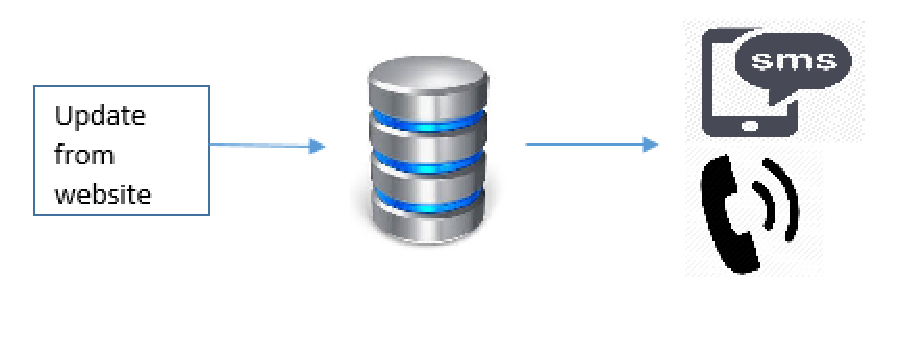
\includegraphics[width=.45\textwidth]{fig/updatefrm.eps}
	\caption{ update from website }
	\label{Figure:update}
\end{figure}


\subsection{Minimum distance calculation}
We determine the optimal route to the nearest shelter and show it to the application and in case of the non-android user we just give them the placement of the nearest shelter. If figure \ref{Figure:optimal} subscriber gets a disaster awareness message form the system. The system will send nearest shelter information. Here if we calculate Euclidean Distance \cite{krislock2012euclidean} we find nearest shelter point is B. But that existing path is so far than path A. For that reason we use trajectory partitioning method\cite{lee2007trajectory} to calculate distance between two places. Trajectory partitioning means path partitioning, which is very important because propose algorithm has used sub-trajectories. 

\begin{figure}[htp]
	\centering
		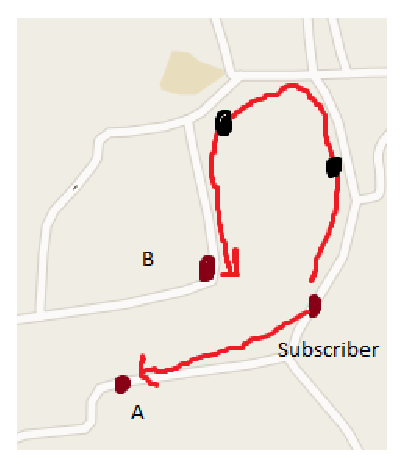
\includegraphics[width=.35\textwidth]{fig/optimalp.eps}
	\caption{ Calculation of nearest shelter place. }
	\label{Figure:optimal}
\end{figure}


\begin{figure}[ht]
	\centering
		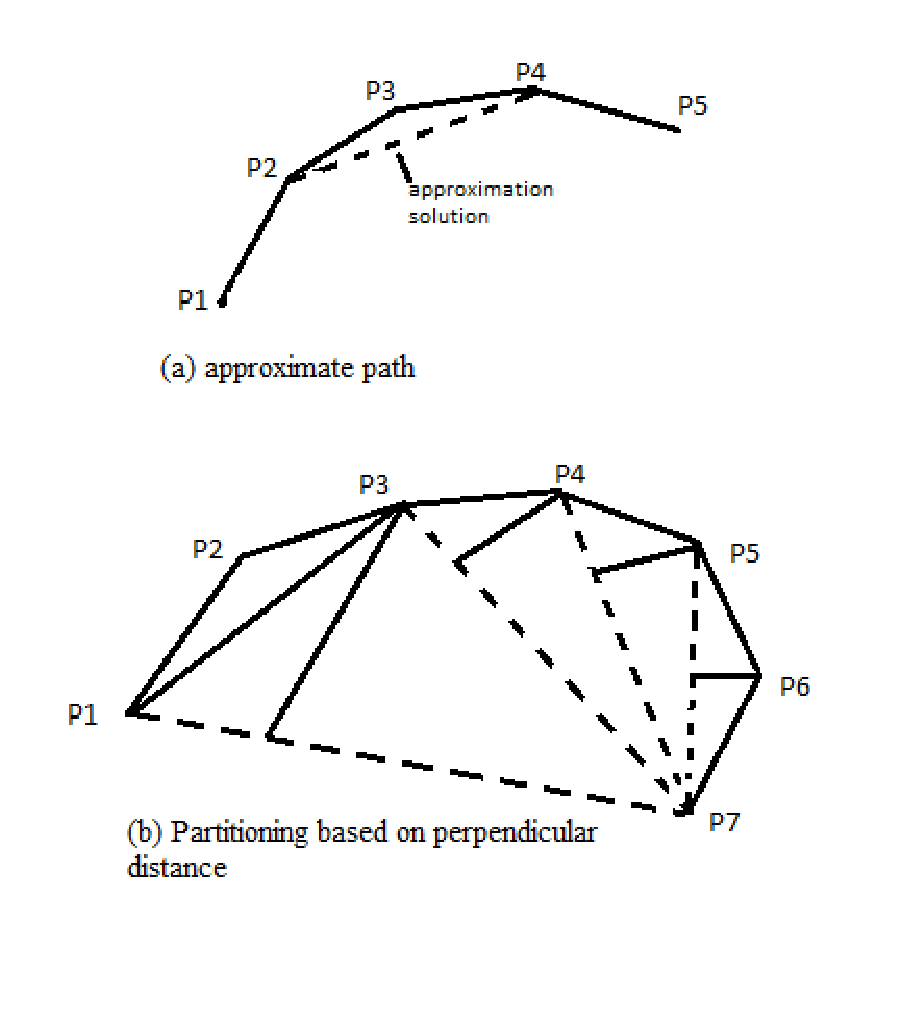
\includegraphics[width=.5\textwidth]{fig/trajectory.eps}
	\caption{Calculate Minimum distance function for path shelter}
	\label{Figure:MDLCOST}
\end{figure}
 

For partitioning, we first took the starting and ending point of the route. Then from the starting point we move towards using the trajectory points. In the first trajectory point we measured the perpendicular distance with respect to the line which was drawn from the starting and ending point of the route. We used equation \ref{eq:perpend} to measure the perpendicular distance where $(m,n)$ is the coordinate of the trajectory point, $d$ is the perpendicular distance, and $Ax+By+c=0$ is the equation of the line. Then we check the perpendicular distance to the given limit to check whether it would need to partition the trajectory. If the distance is greater than the given limit, we would partition the trajectory into two parts. Figure \ref{Figure:MDLCOST}(a) shows the approximate solution structure. The other partition will replace the existing line which was used to measure the perpendicular distance. Then from every point we follow these steps and determine the trajectory path and store them in the array and finally shows the result. In figure \ref{Figure:MDLCOST}(b) $P3$ trajectory partitioned into two parts.Then we measure the perpendicular distance for the partitions. For left partition the distance is lower than the given limit, so we can take the partition as an approximate solution and store the result in an array. 

\begin{equation}
d = \frac{|Am+Bn+c|}{\sqrt{A^2+B^2}}
\label{eq:perpend}
\end{equation}



Algorithm \ref{alg:mindistance} and \ref{alg:distance} shows the procedure to determine the distance of the trajectory path from the starting point to ending point. In algorithm \ref{alg:mindistance} for every trajectory $tr_i$, we found the minimum distance of the subscriber $u$. Then we select the start point $tr_i$$[pos]$. And call the $distance$ function explained in the algorithm \ref{alg:distance}. Then we recommend a shelter point to the subscriber $u$.
In algorithm \ref{alg:distance} for each $position$ and for each starting point $SP_i$ we check the perpendicular distance with the given limit. If the distance is greater than the given limit, then we can call the $distance$ function twice for the left and right partition. If the perpendicular distance is lower than the limit we took the approximate solution and store the result. Lastly it calculates the total distance from the two partition or with the approximate distance for each trajectory and return the result in the algorithm \ref{alg:distance}.



\begin{table}[htp]
\centering
\caption{Alert Classification}

\begin{tabular}{|l|c|c|}
\hline
Disaster & SMS & Voice Alert \\
\hline
Rainfall & Yes & Yes \\
\hline
Heavy Rainfall & Yes & Yes  \\
\hline

Cyclone & Yes & Yes \\
\hline

Wildfire & Yes & Yes\\
\hline

Flood & Yes & Yes\\
\hline
\end{tabular}
\label{tab:alertclass}
\end{table}


\subsection{Predicting weather}
Smart disaster notification system stores weather data into database. Then it apply machine learning techniques to find pattern from these data. After that it predicts whether there will be any disaster by using real-time data. It here predicts rain/ flood possibility by analyzing weather statistics data. It uses Naive Bayes algorithm to find the pattern from the weather statistics data. Equation \ref{eq:naive} is for Naive Bayes classifier. 


\begin{equation}
P(C_i|X) = \frac{P(X|C_i)P(C_i)}{P(X)}
\label{eq:naive}
\end{equation}

Where $X$ represents a vector and $C$ represents class.

\subsection{Sending notification}
After getting updates from websites minimum distance is calculated and then a notification is sent to the subscriber who already registered in the database. This notification is both audio and text message because subscriber can be blind.


\begin{figure}[htp]
	\centering
		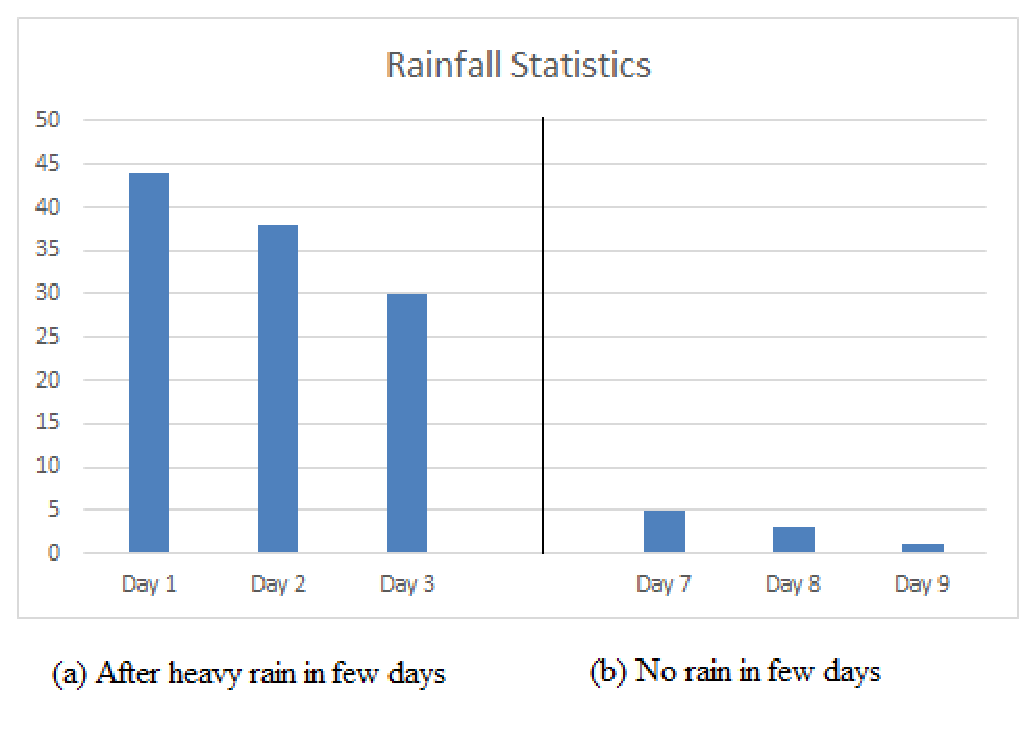
\includegraphics[width=.49\textwidth]{fig/floodjs.eps}
	\caption{ Weather Update statistics view.  }
	\label{Figure:rainfall}
\end{figure}



\subsection{Location tracking of victim}
At the time of disaster, subscribers are in the middle of it. Then for rescue, this application determines the victim’s location by using GPS for android or triangulate location using mobile network for non-android phone and send back the data to the rescue center.




\begin{figure*}[htp]
	\centering
		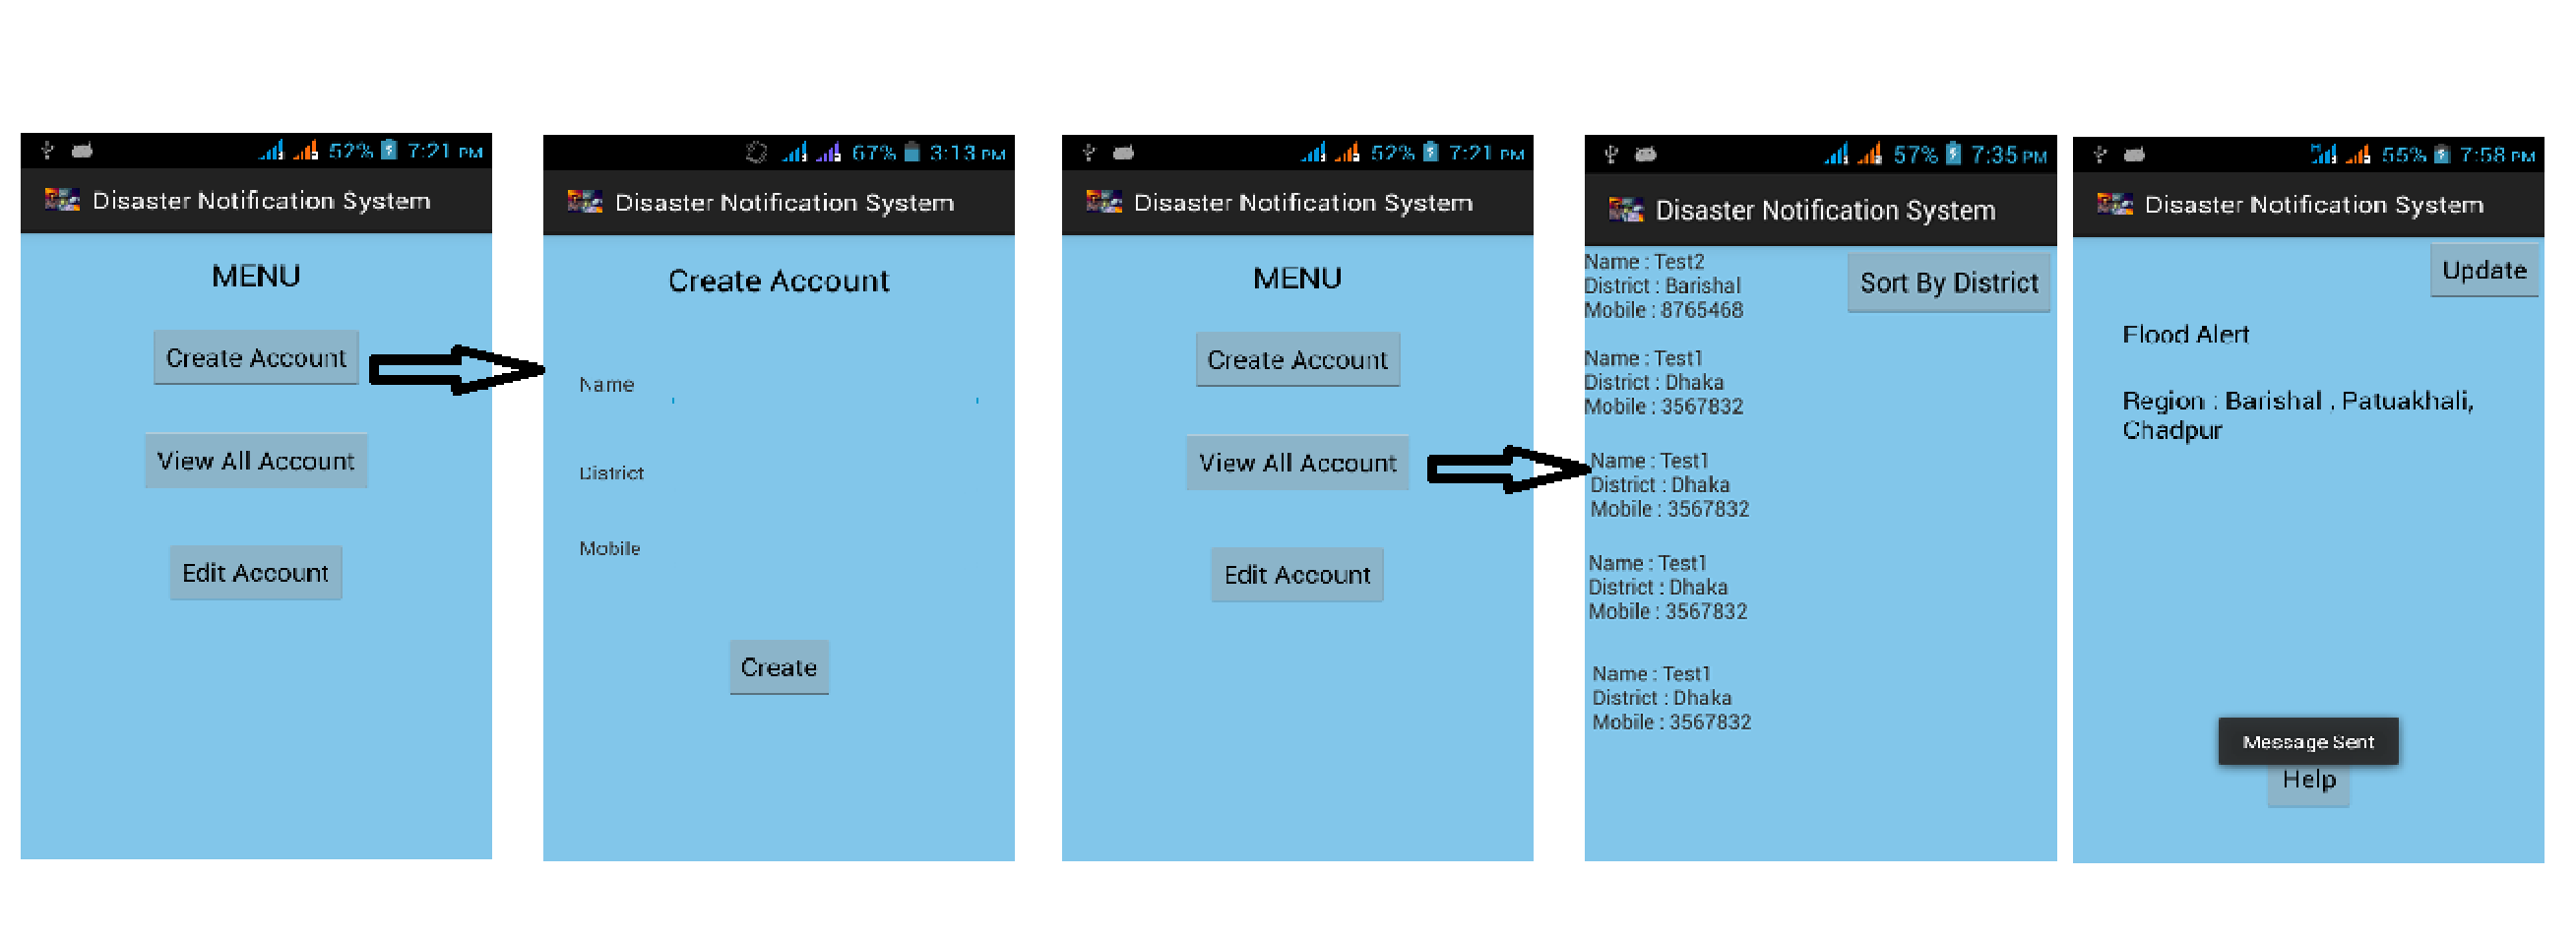
\includegraphics[width=.95\textwidth]{fig/scrnn.eps}
	\caption{ Application Demonstration. }
	\label{Figure:application}
\end{figure*}




\section {Implementation}
\label{implementation}

In our implementation, we have used android based smart technology. For alerting people we first insert their data into the application’s database. In database, subscriber locations are also saved. Then the application communicates with the server. Determining the kind of situation server responses with a JSON file containing the weather information. This application reads the JSON file and convert the data into a message which would be sent to the people whose data are in the database. If JSON file gets some disaster like as Cyclone, Flood, Wildfire it sends SMS or voice call to the subscribers.   


\subsection{Database Design}

This is an Android application so we used Sqlite database\cite{junyan2009application}. This database contains three attributes which are subscriber name, mobile number and region. The attribute mobile number acts as a primary key because mobile number is unique for subscribers.  In the weather server, we create database tables for storing the weather status and to store the shelters position. 

\subsection{Application Testing}

Figure \ref{Figure:rainfall}(a) shows that statistics of rain of some days. By running naive bayes algorithm it predicts that heavy rainfall may cause flood and it can affect some areas. So the JSON file points to those possible affected areas. If the statistics show no promising situation of disaster system, it points to no warning in figure \ref{Figure:rainfall}(b). The system searchs if there is anyone exist in affected regions, it sends them the alert. By this only the affected people get alerts, not all the people in the database. Table \ref{tab:alertclass} shows the overview of the alert classification.


Figure \ref{Figure:application} shows inner looking of the application. For inserting data into the database users need to press the create account button and give the information. After completing registration, data of the people are saved in the database. User also can edit or delete account information by choosing Edit Account Menu. After pressing the Edit Account button there are two options edit account or delete accounts. If user wants to edit account, then user has to provide the mobile number which is unique (primary key) and then edit the information. For deleting account user have to again give the mobile number. Then systems will search the database corresponding that mobile number and will delete that information. When apps requests for weather updates, website calculates the situation of the disaster and make JSON report according to the condition of the weather.

%\section{Discussion}
%\label{discussion}


\begin{algorithm}
\caption{MinDistance (TR, U)}
\label{alg:mindistance}
\begin{algorithmic}[1]
\For{each $u$ \Pisymbol{psy}{206} $U$ }
\For{each $tr$($i$) \Pisymbol{psy}{206} $TR$ }
\State Find minDistance $u$ to $tr$($i$)
\State Select startPoint = $tr$($i$)$[pos]$
\State minDistance = Distance ($tr$($i$) , $SP$)
\EndFor
\EndFor
\State Recommand minDistance up to $u$
\end{algorithmic}
\end{algorithm}



\begin{algorithm}
\caption{Distance ($tr_i$$[pos]$, SP)}
\label{alg:distance}
\begin{algorithmic}[1]
%\Procedure{CH\textendash Election}{}
\For{each $psoition$ \Pisymbol{psy}{206} $tr_i$$[pos]$ }
\For{each $SP_i$ \Pisymbol{psy}{206} $SP$ }
\State Check PD with the given limit /* PD = Perpendicular Distance */ 
\State Distance ($tr_i$$[pos]$, $i$)
\State Distance ($i$, $SP_i$)
\EndFor
\State Calculate total distance
\EndFor
\end{algorithmic}
\end{algorithm}




\section {Result}
\label{result}

In our system, we have warned people before disaster via sms also told them the optimum route to the shelter. A lot of works exists with the same types of feature but our contribution is we have used partition based trajectory distance where others system used Dijkstra's algorithm or euclidean distance to measure the optimum path to the shelter position. A comparison of our works with other works is showed in table \ref{tab:comparison}.

\begin{table}[htp]
\centering
\caption{Comparison with other works }

\begin{tabular}{|l|c|c|c|c|}
\hline
Research& Alert & Tell user  & Algorithm used  & Weather  \\
Work & People & shelter & for measuring & Prediction\\
& & position & optimal path & \\
\hline
Our Work & Yes & Yes & Partition based& Yes \\
& & & trajectory & \\
& & &distance & \\
\hline

Marius et. al\cite{cioca2008sms} & Yes & No & No & No \\
\hline
Jovilyn et. al\cite{fajardo2010implementation} & Yes & Yes & Euclidean & No \\
\hline

Amit et. al\cite{amit2014} & Yes & Yes & Dijkstra's & No \\
\hline

Gamini et. al\cite{jayasinghe2006gsm} & Yes & No & No & No \\
\hline

Rahman et. al\cite{rahman2012location} & Yes & Yes & Eucledian & No \\
\hline

\end{tabular}
\label{tab:comparison}
\end{table}

Table \ref{tab:resultclass} shows the comparison between euclidean distance and trajectory distance. We can see that for every test case the Euclidean distance is smaller than the trajectory distance. Because Euclidean distance only calculates through the direct path using co-ordinate of two places. But there may not be direct paths from those two places. In this case, trajectory distance is more accurate than the Euclidean distance. Hence, we can calculate the nearest shelter and recommend the subscriber. The approach which Amit Gosavi \cite{amit2014} took, used Dijkstra's algorithm to find the nearest shelter where as we have used partition based trajectory distance. Also our application gives weather prediction using real-time and archived weather data.



\begin{table}[htp]
\centering
\caption{Trajectory Path Result}

\begin{tabular}{|l|c|c|}
\hline
Test Case & Euclidean Distance & Calculated Trajectory Distance \\
\hline
1 & 1.95 Km & 5.1 Km \\
\hline
2 & 0.18 Km & 0.19 Km  \\
\hline

3 & 1.07 Km & 1.39 Km \\
\hline

4 & 3.46 Km & 3.96 Km\\
\hline

\end{tabular}
\label{tab:resultclass}
\end{table}



\section{Discussion and Conclusions}
\label{conclusion}

Disaster do not consider any geographical boundary. To minimize the losses in these natural phenomena we should prepare ourselves. Android technology allows us to get information from websites easily. And disaster alert should be a solution to help and give necessary instruction to people that would save many human lives. This application gives alert before disaster like heavy rain, flood, wildfire and so on. This also calculates the optimal route to the nearest shelter. Also it predicts flood by analyzing previous weather data. 

In future work we will try to predict cyclone by using previous cyclonic weather data. We will try to create awareness of other unexpected disaster that happen very quickly like Tsunami and Earthquake.  


%\section*{Acknowledgment}
%The authors are grateful to the anonymous reviewers for their comments that improved the quality of our paper. This research was supported by the research fund of Bangabandhu
%Sheikh Mujibur Rahman Science and Technology University, Bangladesh. Sajal Halder is the corresponding author.

% (used to reserve space for the reference number labels box)


%\begin{thebibliography}{1}
%
%\bibitem{IEEEhowto:kopka}
%H.~Kopka and P.~W. Daly, \emph{A Guide to \LaTeX}, 3rd~ed.\hskip 1em plus
  %0.5em minus 0.4em\relax Harlow, England: Addison-Wesley, 1999.
%
%\end{thebibliography}

%\bibliographystyle{IEEETran}
\bibliographystyle{unsrt}
\balance
\bibliography{hello}

\end{document}

